%% setup
\documentclass[multi=page]{standalone}
%
%% tikzipicture
\usepackage{tikz}
%
%% to use sans serif font
\renewcommand{\familydefault}{\sfdefault}
\usepackage{helvet}
% \usepackage{mathptmx} (times)


\begin{document}

%%%%%%%%%%%%%%
%% COMMANDS %%
%%%%%%%%%%%%%%

%% figurePage
%% goal: create a new figure page
% @arg1 - scaling of content of figure page
% @arg2 - content of figure page
\newcommand{\figurePage}[2]{
	\begin{page}
		\begin{tikzpicture}
			\node [minimum size = 18cm,rectangle,fill=white] at (0,0) {}; %% frame
			\node [scale=#1] at (0,0) {
				#2
			};
		\end{tikzpicture}
	\end{page}
}

%% cropMask
%% goal: create a crop mask function
% @arg1 - width of mask
% @arg2 - height of mask
% @arg3 - x center of mask content
% @arg4 - y center of mask content
% @arg5 - x position of mask 
% @arg6 - y position of mask
% @arg7 - content of mask
\newcommand{\cropMask}[7]{
	\node [minimum width=#1,minimum height=#2,path picture={
			\node at (#3,#4) {
				#7
			};
		}] at (#5,#6) {};
}

%
%%%

%%%%%%%%%%%%%%%%%%%%%
%% FIGURES METHODS %%
%%%%%%%%%%%%%%%%%%%%%

%% new figure
\figurePage{.9}{
	\includegraphics[page=1]{"supporting/DPhil - Ecological interactions paper - 13-04-2022 - v0_1.pdf"}
}

%
%%%

%%%%%%%%%%%%%%%%%
%% FIGURES POC %%
%%%%%%%%%%%%%%%%%


%% TS LV %%

%% new figure
\figurePage{.9}{
	\includegraphics[page=1]{"scripts/case_studies/NODE_GM_LV/out/fig_crossVal_p.pdf"}
}

%% new figure
\figurePage{.9}{
	\includegraphics[page=1]{"scripts/case_studies/NODE_GM_LV/out/fig_predictions_o.pdf"}
}

%% new figure
\figurePage{.9}{
	\includegraphics[page=1]{"scripts/case_studies/NODE_GM_LV/out/fig_predictions_p.pdf"}
}


%% TS 1 %%

%% new figure
\figurePage{.9}{
	\includegraphics[page=1]{"scripts/case_studies/NODE_GM_TS_1/out/fig_crossVal_p.pdf"}
}

%% new figure
\figurePage{.9}{
	\includegraphics[page=1]{"scripts/case_studies/NODE_GM_TS_1/out/fig_predictions_o.pdf"}
}

%% new figure
\figurePage{.9}{
	\includegraphics[page=1]{"scripts/case_studies/NODE_GM_TS_1/out/fig_predictions_p.pdf"}
}


%% TS 2 %%

%% new figure
\figurePage{.9}{
	\includegraphics[page=1]{"scripts/case_studies/NODE_GM_TS_2/out/fig_crossVal_p.pdf"}
}

%% new figure
\figurePage{.9}{
	\includegraphics[page=1]{"scripts/case_studies/NODE_GM_TS_2/out/fig_predictions_o.pdf"}
}

%% new figure
\figurePage{.9}{
	\includegraphics[page=1]{"scripts/case_studies/NODE_GM_TS_2/out/fig_predictions_p.pdf"}
}


%% TS 3 %%

%% new figure
\figurePage{.9}{
	\includegraphics[page=1]{"scripts/case_studies/NODE_GM_TS_3/out/fig_crossVal_p.pdf"}
}

%% new figure
\figurePage{.9}{
	\includegraphics[page=1]{"scripts/case_studies/NODE_GM_TS_3/out/fig_predictions_o.pdf"}
}

%% new figure
\figurePage{.9}{
	\includegraphics[page=1]{"scripts/case_studies/NODE_GM_TS_3/out/fig_predictions_p.pdf"}
}

%
%%%

%%%%%%%%%%%%%%%%
%% DISCUSSION %%
%%%%%%%%%%%%%%%%

%% new figure
\figurePage{.9}{
	\includegraphics[page=2]{"supporting/DPhil - Ecological interactions paper - 13-04-2022 - v0_1.pdf"}
}

%
%%%

\end{document}
